\documentclass{fkpresentation}

\setcounter{errorcontextlines}{999}
% Information to be included in the title page:
\title{\textmd{The Euler-Lagrange Equation}}
\author{Forest Kobayashi}
\institute{Harvey Mudd College}
\date{April 1st, 2018}

\usetikzlibrary{external}
\tikzexternalize

\begin{document}
\frame{\titlepage}
\section{Motivation}
\begin{frame}

\end{frame}

\section{Proof Sketch}

% Function:
% z = 3 * (1-x)^2 * exp(-(x^2) - (y+1)^2) - 10 * (x/5 - x^3 - y^5) * exp(-x^2 -
% y^2) - 1/3 * exp(-(x+1)^2 - y^2)

\begin{frame}
  \begin{figure}[h]
    \centering
    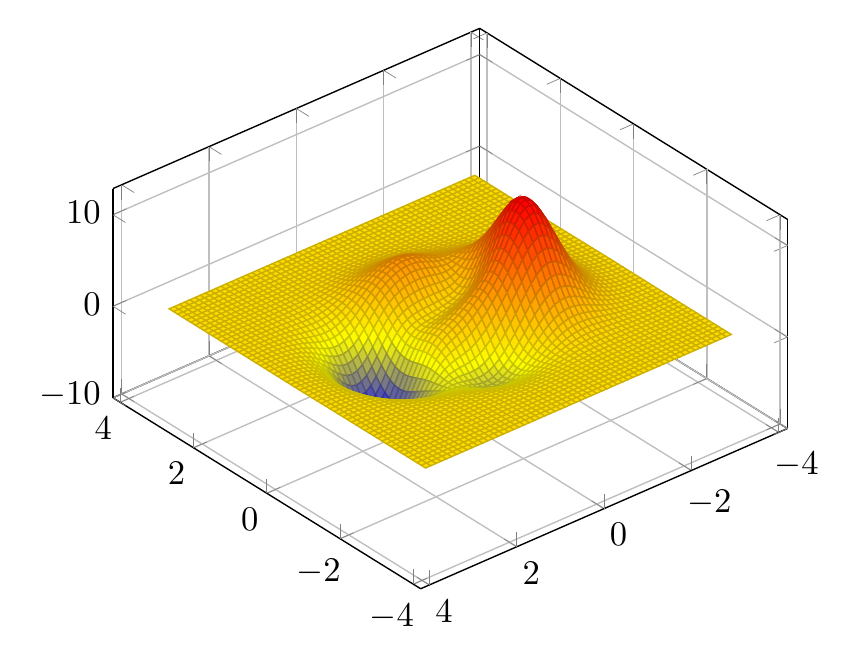
\begin{tikzpicture}[
      scale=1.25,
      declare function = {
        a(\x, \y) = 3*(1-\x)^2 * exp(-(\x^2)-(\y+1)^2);
        b(\x, \y) = -10*(\x/5 - \x^3 + \y^5) * exp(-\x^2 - \y^2);
        c(\x, \y) = -exp(-(\x+1)^2 - \y^2)/3;
        Z(\x, \y) = a(\x,\y) + b(\x,\y) + c(\x,\y);
        % Z(\x, \y) = 3*(1-\x)^2 * exp(-(\x^2)-(\y+1)^2) - 10 * (\x/5 - \x^3 + \y^5) *
        % exp(-\x^2 - \y^2) - exp(-(\x+1)^2 - \y^2)/3;
      }
      ]
      \begin{axis}[
        view={230}{50},
        % axis lines=center,
        enlargelimits,
        % tick align=inside,
        domain=-3.5:3.5,
        samples=60,
        grid=major,
        % minor tick num=5
        ]
        \addplot3 [surf] {Z(x,y)};
      \end{axis}
    \end{tikzpicture}
  \end{figure}
\end{frame}

\begin{frame}
  \begin{figure}[h]
    \centering
    \begin{tikzpicture}
      \pgfmathsetmacro{\xmin}{-1};
      \pgfmathsetmacro{\ymin}{-1};
      \pgfmathsetmacro{\xmax}{6};
      \pgfmathsetmacro{\ymax}{5};

      \pgfmathsetmacro{\extraforaxes}{.2};

      \pgfmathsetmacro{\epsilon}{.1};

      \draw[->] (\xmin,0) -- (\xmax+\extraforaxes, 0) node[below] {$x$};
      \draw[->] (0,\ymin) -- (0, \ymax+\extraforaxes) node[left] {$y$};

      \draw[domain=1.5:5.5, smooth, variable=\x, blue] plot ({\x-.5},
      {-1.7 + \x * (3.31667 + (-0.9 + 0.0833333 * \x) * \x)});

      \node[
        circle,
        draw=black,
        fill=white,
        inner sep=0pt,
        minimum size=5pt
        ] (y0) at (1, 1.56875) {};

      \node[
        circle,
        draw=black,
        fill=white,
        inner sep=0pt,
        minimum size=5pt
        ] (y1) at (5, 3.18126) {};

      % \draw[domain=\xmin:\xmax, smooth, variable=\x, blue] plot ({\x}, )

      % \draw[scale=0.5,domain=-3:3,smooth,variable=\x,blue] plot ({\x}, {\x*\x});
      % \draw[scale=0.5,domain=-3:3,smooth,variable=\y,red]  plot ({\y*\y}, {\y});
    \end{tikzpicture}
  \end{figure}
\end{frame}


% \section{Bibliography}
% \begin{frame}
%   \frametitle{References}
%   \bibliographystyle{alpha}
%   % \bibliographystyle{IEEE}
%   \bibliography{aha.bib}
% \end{frame}

\end{document}


%%% Local Variables:
%%% TeX-master: t
%%% TeX-engine: default-shell-escape
%%% TeX-command-extra-option: -pdf
%%% End: